
%\begin{figure}[t]
%\centering
%\includegraphics[scale=1,clip]{figure/n2n.eps}\vspace*{-3ex}
% \caption{Merging technique}\vspace*{-3.5ex}
% \label{fig:n2n}
%\end{figure}

\section{Discussion and Future Work}
\label{sec:discuss}

We next discuss some known limitations of our approach and describe how we address these limitations in our future work.

\textbf{Detecting more behavior differences.} Our results show that TeMAPI does not achieve 100\% coverage for a few classes. Therefore, TeMAPI may fail to reveal some differences. To detect more behavior differences, we plan to explore the following directions in our future work. (1) To test API methods without return values, we plan to test side effects or mock objects. (2) To test API methods that return random values, we plan to verify the distribution of their returned values. (3) To test methods that require file interactions, we plan to generate test cases based on the Java Compatibility Kit (JCK)\footnote{\url{http://jck.dev.java.net}}, where standard method-call sequences and files are prepared. (4) We also plan to leverage other tools such as Cute~\cite{koushik:cute} and JPF~\cite{visser2003mcp} to generate more test cases.

\textbf{Testing translation of code structures.} As shown in our evaluations, translation tools may fail to translate complicated code structures. We observe that other translation tools can encounter similar issues. In our future work, we plan leverage the idea of Daniel \emph{et al.}~\cite{daniel2007automated}'s approach to address these issues. They propose an approach that tests refactoring engines by comparing their refactored results, given the same generated abstract syntax trees. We plan to leverage their idea to test code structures for translation tools by comparing the translation results, given the same code structures.

%\textbf{Testing API mapping of single language.} We find that many existing approaches translate applications within single languages. For example, twinning~\cite{nita2010using} translates applications based on mapping relations of API invocations from different API libraries, and CatchUp!~\cite{henkel2005catchup} translates applications based on mapping relations of API invocations from different versions. In future work, we plan to adapt our approach to test mapping relations of API invocations within single languages. 